\whiteBGstarBegin

\begin{enumerate}[label=\bfseries Câu \arabic*:]
	
	\item \mkstar{1}
	
	\cauhoi{
		Phát biểu nào sau đây \textbf{không} đúng khi nói về từ thông?
		
		\begin{mcq}
			\item Biểu thức định nghĩa của từ thông là $\Phi=B\cdot S\cdot \cos \alpha$. 
			\item Đơn vị của từ thông là vêbe (Wb).
			\item Từ thông là một đại lượng đại số.
			\item Từ thông là một đại lượng có hướng. 
		\end{mcq}
	}
	
	\loigiai{\textbf{Đáp án: D.}
		
		Từ thông là một đại lượng vô hướng.
		
		
	}
	\item \mkstar{1}
	
	\cauhoi{Đơn vị của từ thông có thể là
		
		\begin{mcq}(2)
			\item tesla trên mét $(\text{T/m})$.
			\item tesla nhân với mét $(\text{T.m})$.
			\item tesla nhân mét bình phương $(\text{T.m}^2)$.
			\item tesla trên mét bình phương $(\text{T/m}^2)$.
		\end{mcq}
	}
	\loigiai{\textbf{Đáp án: C.}
		
		Đơn vị của từ thông có thể là tesla nhân mét bình phương $(\text{T.m}^2)$.
		
		
	}
	\item \mkstar{1}
	
	\cauhoi{
		Công thức định luật Fa-ra-đây về cảm ứng điện từ là 	
		\begin{mcq}(4)
			\item $e=-\dfrac{\Delta \Phi}{\Delta t}$.
			\item $e=-\dfrac{\Delta \Phi}{\Delta t^2}$.
			\item $e=-\Delta \Phi\cdot \Delta t$.
			\item $e=-\Delta \Phi\cdot \Delta t^2$.
		\end{mcq}
	}
	\loigiai{\textbf{Đáp án: A.}
		
		Công thức định luật Fa-ra-đây về cảm ứng điện từ là $e=-\dfrac{\Delta \Phi}{\Delta t}$.
		
		
	}
	\item \mkstar{2}
	
	\cauhoi{Từ thông qua một mạch điện kín phụ thuộc vào
		\begin{mcq}(1)
			\item tiết diện của dây dẫn làm mạch điện.
			\item điện trở của dây dẫn làm mạch điện.	
			\item khối lượng của dây dẫn làm mạch điện.	
			\item hình dạng, kích thước của mạch điện.
		\end{mcq}
	}
	\loigiai{\textbf{Đáp án: D.}	
		
		Từ thông qua một mạch điện kín phụ thuộc vào hình dạng, kích thước của mạch điện.
		
		
	}
	\item \mkstar{2}
	
	\cauhoi{
		Một khung dây phẳng được đặt trong mặt phẳng hình vẽ, các đường sức của từ trường đều có phương vuông góc với mặt phẳng hình vẽ và hướng từ trong ra. Xác định chiều của dòng điện cảm ứng trong khung khi giảm độ lớn cảm ứng từ của từ trường.
		
		\begin{mcq}
			\item Ngược chiều kim đồng hồ.
			\item Ban đầu  theo chiều kim đồng hồ, sau đó đổi chiều.
			\item Ban đầu ngược chiều kim đồng hồ, sau đó đổi chiều
			\item Theo chiều kim đồng hồ.
		\end{mcq}	
	}
	\loigiai{\textbf{Đáp án: A.}
		
		Dựa vào định luật Len-xơ về chiều dòng điện cảm ứng, chiều của dòng điện cảm ứng trong khung khi giảm độ lớn cảm ứng từ của từ trường sẽ chạy ngược chiều kim đồng hồ.
		
		
	}
	\item \mkstar{2}
	
	\cauhoi{
		Một khung dây hình tròn có diện tích $2\ \text{cm}^2$ đặt trong từ trường, các đường sức từ xuyên vuông góc với khung dây. Hãy xác định từ thông xuyên qua khung dây, biết rằng $B=5\cdot 10^{-2}\ \text{T}$.  
		
		\begin{mcq} (4)
			\item $10^{-5}\ \text{Wb}$.
			\item $2\cdot 10^{-5}\ \text{Wb}$.
			\item $3\cdot 10^{-5}\ \text{Wb}$.
			\item $4\cdot 10^{-5}\ \text{Wb}$.
			
		\end{mcq}
	}
	
	\loigiai{\textbf{Đáp án: A.}
		
		Từ thông xuyên qua khung dây là $\Phi=B\cdot S\cdot \cos \alpha=10^{-5}\ \text{Wb}$ .
		
		
	}
	\item \mkstar{2}
	
	\cauhoi{
		Một khung dây hình vuông có cạnh dài 5 cm, đặt trong từ trường đều cảm ứng từ $B=2\cdot 10^{-2}\ \text{T}$, khung dây tạo với các đường sức một góc $30^\circ$. Hãy tính từ thông xuyên qua khung dây.
		\begin{mcq}(4)
			\item $\text{6,25}\cdot 10^{-5}\ \text{Wb}$.
			\item $\text{2,5}\cdot 10^{-5}\ \text{Wb}$.
			\item $\text{10,08}\cdot 10^{-5}\ \text{Wb}$.
			\item $\text{1,25}\cdot 10^{-5}\ \text{Wb}$.
		\end{mcq}	
	}
	
	\loigiai{\textbf{Đáp án: B.}
		
		Mặt phẳng khung dây làm thành với $\vec{B}$ góc $30^\circ$ nên góc giữa $\vec{B}$ và pháp tuyến $\vec{n}$ là $$\alpha=90^\circ -30^\circ=60^\circ$$
		
		Diện tích hình vuông là $$S=a^2=\text{2,5}\cdot 10^{-3}\ \text{m}^2$$
		
		Từ thông xuyên qua khung dây là $$\Phi=BS\cos \alpha=\text{2,5}\cdot 10^{-5}\ \text{Wb}$$
		
		
	}
	\item \mkstar{2}
	
	\cauhoi{
		Từ thông $\Phi$ qua một khung dây biến đổi, trong khoảng thời gian $\text{0,2}\ \text{s}$ thì từ thông tăng từ $\text{0,3}\ \text{Wb}$ lên đến $\text{2,3}\ \text{Wb}$. Suất điện động cảm ứng xuất hiện trong khung có độ lớn bằng
		\begin{mcq}(4)
			\item $\text{0,1}\ \text{V}$.
			\item $\text{2,2}\ \text{V}$.
			\item $\text{0,4}\ \text{V}$.
			\item $\text{10}\ \text{V}$. 
		\end{mcq}
	}
	
	\loigiai{\textbf{Đáp án: D.}
		
		Suất điện động cảm ứng xuất hiện trong khung có độ lớn bằng
		
		$$|e|=\left| -\dfrac{\Delta \Phi}{\Delta t}\right| =\text{10}\ \text{V}$$
		
		
	}
	\item \mkstar{2}
	
	\cauhoi{Đối với một cuộn dây, hệ số tự cảm phụ thuộc vào
		
		\begin{mcq}(2)
			\item cảm ứng từ trong lòng cuộn dây.
			\item cấu tạo của cuộn dây.
			\item cường độ dòng điện qua cuộn dây.
			\item từ thông qua cuộn dây.
		\end{mcq}
	}
	
	\loigiai{\textbf{Đáp án: B.}
		
		Đối với một cuộn dây, hệ số tự cảm phụ thuộc vào cấu tạo của cuộn dây.
		
		
	}
	\item \mkstar{2}
	
	\cauhoi{
		Năng lượng từ trường của một ống dây sẽ thay đổi như thế nào nếu cường độ dòng điện qua ống dây tăng lên hai lần?
		
		\begin{mcq}(2)
			\item Tăng lên bốn lần.	
			\item Giảm đi bốn lần.
			\item Giảm đi hai lần.
			\item Tăng lên hai lần.
		\end{mcq}
	}
	
	\loigiai{\textbf{Đáp án: A.}
		
		Năng lượng từ trường của một ống dây
		
		$$W=\dfrac{1}{2}L\cdot i^2, W'=\dfrac{1}{2}L\cdot i'^2$$
		
		Mà $i'=2i$ nên $W'=4W$.
		
		
	}
	\item \mkstar{2}
	
	\cauhoi{Hãy xác định suất điện động cảm ứng của khung dây, biết rằng trong khoảng thời gian $\text{0,5}\ \text{s}$, từ thông giảm từ $\text{1,5}\ \text{Wb}$ đến $0$.
		\begin{mcq}(4)
			\item 6 V.
			\item 3 V. 
			\item 12 V.
			\item 1 V.
		\end{mcq}
	}
	
	\loigiai{\textbf{Đáp án: B.}
		
		Suất điện động cảm ứng của khung dây là $$e=\left| \dfrac{\Delta \Phi}{\Delta t}\right| =3\ \text{V}$$
		
		
	}
	\item \mkstar{3}
	
	\cauhoi{
		Từ thông giảm từ $\text{1,5}\ \text{Wb}$ đến $2\ \text{Wb}$ trong khoảng thời gian $\Delta t$ thì suất điện động cảm ứng của khung dây trong khung dây có giá trị là $5\ \text{V}$.  Tìm khoảng thời gian $\Delta t$ đó.
		\begin{mcq}(4)
			\item $\text{0,1}\ \text{s}$.
			\item $\text{0,2}\ \text{s}$.
			\item $\text{0,3}\ \text{s}$. 
			\item $\text{0,5}\ \text{s}$. 
		\end{mcq}
	}
	
	\loigiai{\textbf{Đáp án: A.}
		
		Khoảng thời gian $\Delta t$
		$$e=\left| \dfrac{\Delta \Phi }{\Delta t}\right| \Rightarrow \Delta t=\text{0,1}\ \text{s}$$
		
		
	}
	\item \mkstar{3}
	
	\cauhoi{ Từ thông qua một khung dây biến thiên theo thời gian theo phương trình: $\Phi=\text{0,05}t\ \text{Wb}$, trong đó $\Phi$ là kí hiệu của từ thông, $t$ là kí hiệu của thời gian.Tính độ lớn suất điện động cảm ứng trong mạch trong khoảng thời gian từ $t_1=1\ \text{s}$ đến $t_2=3\ \text{s}$.
		
		\begin{mcq}(4)
			\item $\text{0,05}\ \text{V}$.
			\item $\text{0,5}\ \text{V}$.
			\item $\text{0,01}\ \text{V}$.
			\item $\text{0,1}\ \text{V}$.
		\end{mcq}
	}
	
	\loigiai{\textbf{Đáp án: A.}
		
		Tại $t_1=1\ \text{s}$ thì $\Phi_1=\text{0,05}\ \text{Wb}$.
		
		Tại $t_2=3\ \text{s}$ thì $\Phi_1=\text{0,15}\ \text{Wb}$.
		
		Độ lớn suất điện động cảm ứng: 
		$$\left| e_\text{c}\right| =\left| -\dfrac{\Delta \Phi}{\Delta t}\right|=\left| -\dfrac{\Phi_2-\Phi_1}{\Delta t}\right|= \text{0,05}\ \text{V}$$
		
		
	}
	\item \mkstar{3}
	
	\cauhoi{Từ thông qua một khung dây biến thiên theo thời gian theo phương trình: $\Phi=\text{0,05}t\ \text{Wb}$, trong đó $\Phi$ là kí hiệu của từ thông, $t$ là kí hiệu của thời gian. Tính cường độ dòng điện cảm ứng xuất hiện trong khung. Biết điện trở của khung dây bằng $R=5\ \Omega$.  
		\begin{mcq}(4)
			\item $\text{0,05}\ \text{A}$.
			\item $\text{0,01}\ \text{A}$.
			\item $\text{0,5}\ \text{A}$.
			\item $\text{0,1}\ \text{A}$.
		\end{mcq}
	}
	
	\loigiai{\textbf{Đáp án: B.}
		
		Cường độ dòng điện cảm ứng xuất hiện trong khung:
		$$I_\text{c}=\left| \dfrac{e_\text{c}}{R}\right| =\text{0,01}\ \text{A}$$
		
		
	}
	\item \mkstar{3}
	
	\cauhoi{ Một ống dây dài $l = 30\ \text{cm}$ gồm $N = 1000$ vòng dây, đường kính mỗi vòng dây $d = 8\ \text{cm}$ có dòng điện với cường độ $i = 2\ \text{A}$ đi qua. Tính độ tự cảm của ống dây.
		\begin{mcq}(4)
			\item $\text{0,02}\ \text{H}$.
			\item $\text{0,2}\ \text{H}$.
			\item $\text{0,01}\ \text{H}$.
			\item $\text{0,1}\ \text{H}$.
		\end{mcq}
	}
	
	\loigiai{\textbf{Đáp án: A.}
		
		Ta có:
		$$S=\dfrac{\pi\cdot d^2}{4}=\text{1,6}\cdot \pi\cdot 10^{-3}\ \text{m}^2.$$
		Độ tự cảm của ống dây:
		$$L=4\pi \cdot 10^{-7}\cdot \dfrac{N^2}{l}\cdot S=\text{0,02}\ \text{H}$$
		
		
	}
	\item \mkstar{3}
	
	\cauhoi{ Một ống dây dài $l = 30\ \text{cm}$ gồm $N = 1000$ vòng dây, đường kính mỗi vòng dây $d = 8\ \text{cm}$ có dòng điện với cường độ $i = 2\ \text{A}$ đi qua. Thời gian ngắt dòng điện là $t = \text{0,1}$ giây. Tính độ lớn suất điện động tự cảm xuất hiện trong ống dây.
		
		\begin{mcq}(4)
			\item $\text{0,04}\ \text{A}$.
			\item $\text{0,02}\ \text{A}$.
			\item $\text{0,4}\ \text{A}$.
			\item $\text{0,2}\ \text{A}$.
		\end{mcq}
	}
	
	\loigiai{\textbf{Đáp án: C.}	
		
		Độ lớn suất điện động tự cảm: $$\left| e_\text{tc}\right| =\left| -L\dfrac{ \Delta i}{\Delta t}\right| =\text{0,4}\ \text{V}$$
		
		
	}
	\item \mkstar{3}
	
	\cauhoi{Một khung dây dẫn hình vuông, cạnh $a = 10\ \text{cm}$, đặt cố định trong từ trường đều có vectơ cảm ứng từ $\vec{B}$  vuông góc với mặt phẳng khung dây. Ban đầu cảm ứng từ  có giá trị là $\text{0,5}\ \text{T}$; cho cảm ứng từ  tăng đều. Sau thời gian $\text{0,5}\ \text{s}$ thì cảm ứng từ có giá trị gấp $3$ lần ban đầu. Hãy xác định suất điện động cảm ứng xuất hiện trong khung dây trong khoảng thời gian trên.
		
		\begin{mcq}(4)
			\item $\text{0,02}\ \text{V}$.
			\item $\text{0,01}\ \text{V}$.
			\item $\text{0,03}\ \text{V}$.
			\item $\text{0,04}\ \text{V}$.
		\end{mcq}
	}
	
	\loigiai{\textbf{Đáp án: A.}
		
		Độ biến thiên từ thông:
		$$\Delta \Phi=N\cdot \Delta B\cdot S\cdot \cos \alpha=\text{0,01}\ \text{Wb}$$
		
		Suất điện động cảm ứng là $$e_\text{C}=\left|- \dfrac{\Delta \Phi}{\Delta t}\right| =\text{0,02}\ \text{V}$$
		
		
	}
	
	
	\item \mkstar{4}
	
	\cauhoi{  Một khung dây có $60$ vòng dây đặt trong từ trường có độ lớn cảm ứng từ biến thiên theo thời gian như đồ thị (hình bên). 
		
		\begin{center}
			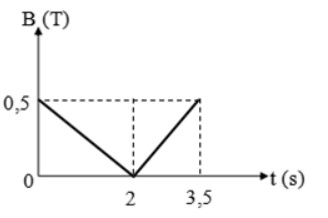
\includegraphics[scale=0.9]{../figs/mid1-hk2-h1.jpg}
		\end{center}
		
		
		Biết rằng đường sức từ hợp với mặt phẳng khung dây một góc $45^\circ$, diện tích mỗi vòng dây là $\text{0,04}\ \text{m}^2$. Độ lớn của suất điện động xuất hiện trong khung dây trong khoảng thời gian $2\ \text{s}$ đầu tiên và trong $\text{1,5}\ \text{s}$ tiếp theo có giá trị lần lượt là
		\begin{mcq}(2)
			\item $\text{0,17}\ \text{V}; \ \text{0,33}\ \text{V}$.
			\item $\text{0,17}\ \text{V}; \ \text{0,23}\ \text{V}$.
			\item $\text{0,27}\ \text{V}; \ \text{0,33}\ \text{V}$.
			\item $\text{0,27}\ \text{V}; \ \text{0,23}\ \text{V}$.
		\end{mcq}
	}
	
	\loigiai{\textbf{Đáp án: A.}
		
		Độ biến thiên từ thông trong khoảng thời gian 2 s đầu là	
		
		
		$$\Delta \Phi_1=-7\cdot 10^{-3}\ \text{Wb}$$
		
		
		Độ lớn của suất điện động trong khoảng thời gian 2 s đầu là	
		$$\left| e_1\right| =\left|-L\cdot \dfrac{\Delta i}{\Delta t} \right|= \text{0,17}\ \text{V}$$
		
		Độ biến thiên từ thông trong khoảng thời gian $\text{1,5}\ \text{s}$ tiếp theo là	
		
		$$\Delta \Phi_2=7\cdot 10^{-3}\ \text{Wb}$$
		
		
		Độ lớn của suất điện động trong khoảng thời gian $\text{1,5}\ \text{s}$ tiếp theo là
		
		$$\left| e_2\right| =\left|-L\cdot \dfrac{\Delta i}{\Delta t} \right|= \text{0,33}\ \text{V}$$
		
		
	}
	\item \mkstar{4}
	
	\cauhoi{Cho dòng điện chạy vào ống dây hình trụ, lõi không khí dài $50\ \text{cm}$, có $1000$ vòng dây và diện tích tiết diện của ống dây là $20\ \text{cm}^2$. Dòng điện biến thiên theo thời gian như đồ thị:
		
		\begin{center}
			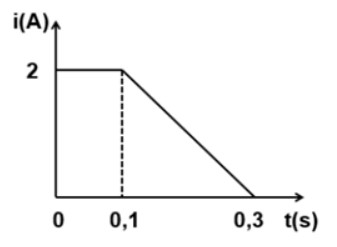
\includegraphics[scale=0.8]{../figs/mid-hk2-h2.jpg}
		\end{center}
		
		Độ lớn suất điện động tự cảm xuất hiện trong ống dây trong các giai đoạn từ $0$ đến $\text{0,1}\ \text{s}$, từ $\text{0,1}\ \text{s}$ đến $\text{0,3}\ \text{s}$ lần lượt là
		\begin{mcq}(2)
			\item $\text{0}\ \text{V}; \ \text{0,02}\ \text{V}$.
			\item $\text{0}\ \text{V}; \ \text{0,05}\ \text{V}$.
			\item $\text{0,05}\ \text{V}; \ \text{0,02}\ \text{V}$.
			\item $\text{0,05}\ \text{V}; \ \text{0}\ \text{V}$.
		\end{mcq}
	}
	
	\loigiai{\textbf{Đáp án: B.}
		
		Từ $0\ \text{s}$ đến $\text{0,1} \text{s}$:
		$$\left| e_\text{c1}\right| =\left| -L\dfrac{\Delta i}{\Delta t}\right| =\text{0}\ \text{V}$$
		
		Từ $\text{0,1}\ \text{s}$ đến $\text{0,3} \text{s}$: $$\left| e_\text{c2}\right| =\left| -L\dfrac{\Delta i}{\Delta t}\right| =\text{0,05}\ \text{V}$$
		
		
	}
	\item \mkstar{4}
	
	\cauhoi{ Một ống dây hình trụ dài gồm $10^3$ vòng dây, diện tích mỗi vòng dây $S = 100\ \text{cm}^2$. Ống dây có điện trở $R = 16\ \Omega$, hai đầu nối đoản mạch và được đặt trong từ trường đều có vectơ cảm ứng từ song song với trục của ống dây và có độ lớn tăng đều $10^{-2}\ \text{T/s}$. Tính công suất tỏa nhiệt của ống dây.
		
		\begin{mcq}(2)
			\item $\text{2,25}\cdot 10^{-3}\ \text{W}$.
			\item $\text{2,25}\cdot 10^{-4}\ \text{W}$.
			\item $\text{6,25}\cdot 10^{-3}\ \text{W}$.
			\item $\text{6,25}\cdot 10^{-4}\ \text{W}$.
		\end{mcq}
	}
	
	\loigiai{\textbf{Đáp án: D.}
		
		Ta có:
		$$\left| e_\text{c}\right| =\left| -\dfrac{\Delta \Phi}{\Delta t}\right|=\left| -\dfrac{N\cdot \Delta B\cdot S}{\Delta t}\right|=\text{0,1}\ \text{V}.$$
		Lại có:
		$$I_\text{c}=\left| \dfrac{e_\text{c}}{R}\right|=\text{0,625}\cdot 10^{-2}\ \text{A}.$$
		Công suất tỏa nhiệt của ống dây
		$$\calP=I^2\cdot R=\text{6,25}\cdot 10^{-4}\ \text{W}.$$
		
		
	}
	
\end{enumerate}

\whiteBGstarEnd

\loigiai{\begin{center}
		\textbf{BẢNG ĐÁP ÁN}
	\end{center}
	\begin{center}	
		\begin{tabular}{|m{2.8em}|m{2.8em}|m{2.8em}|m{2.8em}|m{2.8em}|m{2.8em}|m{2.8em}|m{2.8em}|m{2.8em}|m{2.8em}|}
			\hline
			1.D  & 2.C  & 3.A  & 4.D  & 5.A  & 6.A  & 7.B  & 8.D  & 9.B  & 10.A  \\
			\hline
			11.B  & 12.A  & 13.A  & 14.B  & 15.A  & 16.C  & 17.A  & 18.A  & 19.B  & 20.D \\
			\hline
			
		\end{tabular}
\end{center}}